\chapter{Rapidly-Exploring Random Tree (RRT)}\label{chap:RRT}

\section{General}

The goal of this Thesis was not only to generate a numerical stable, snap optimized polynomial trajectory but also to explore a dense (indoor) environment and plan an aggressive trajectory in between the obstacles. Hence, the Rapidly-Exploring Random Tree (RRT) algorithm is used to find a collision free straight-line solution through the dense environment. The sampling points oft the RRT (or RRT*) algorithm are then used as the vertices in the polynomial optimization.

\section{Algorithm}

\subsection{RRT}

RRT is a computational efficient algorithm to find a path in a high dimensional space by randomly building a space-filling tree. The sampling points are drawn randomly from the sample space and the tree grows incrementally. 
For each new sample the algorithm attempts to build a collision-free connection to the nearest state in the tree. If a collision-free connection is possible the sample and the connection are added to the tree. \newline

The RRT algorithm can be depicted schematically:


\begin{enumerate}
  \item Sample
  \item Find nearest state in the tree
  \item Try to build a collision-free connection to the nearest state
  \item If feasible, add the sampled state and the connection to the tree
\end{enumerate}

\subsection{RRT*}

In contrast to the RRT algorithm the RRT* (or RRT Star) algorithm not only tries to connect to the nearest state in the tree but to several states near the sampled state. The user can define a threshold (on the distance) which defines which states of the tree belongs to the "near states". If there is no state within the user specified range the algorithm attempts to build a collision-free connection to the nearest state in the tree just as the RRT algorithm.  \newline
As a first step, the sampled state is connected to the best state among the near states whereas best means minimum cost/distance. Once the sampled state is added to the tree all the other states among the near states are connected to the sampled state. If the connection is collision-free and the cost of the total path is smaller than the cost of the existing path, the old path is replaced. \newline

The RRT* algorithm can be depicted schematically:


\begin{enumerate}
  \item Sample
  \item Define a set of near states
  \item Try to build a collision-free connection to best state among the near states
  \item Add the sampled state and the connection to the tree 
  \item Try to connect all the other states from the set with the sampled state. 
  \item Replace the old path if the new one has a smaller cost.
  \item If there is no near state in the user specified range apply the RRT algorithm
\end{enumerate}


Because the RRT* algorithm tries to connect to several states each iteration, the procedure of finding a path takes longer and is computationally more expensive. However, solution with lower cost can be found which is more important for most real life applications.

\subsection{Goal State}

As mentioned above, the RRT/RRT* algorithm is based on random samples. Since it is very unlikely that a random sampled state perfectly matches the desired goal state not only a goal state but a goal region is needed. 


\begin{figure}[h]
   \centering
   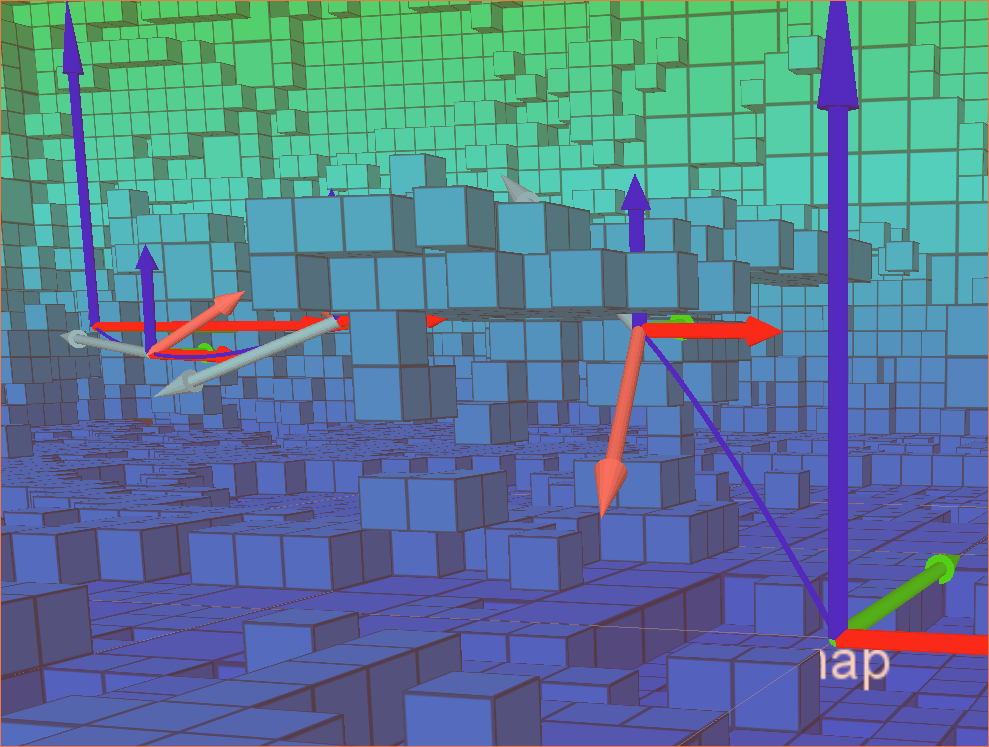
\includegraphics[width=1\textwidth]{pics/initialSolution.png}
   \caption{Ein Bild.}
\end{figure}


\begin{figure}[h]
   \centering
   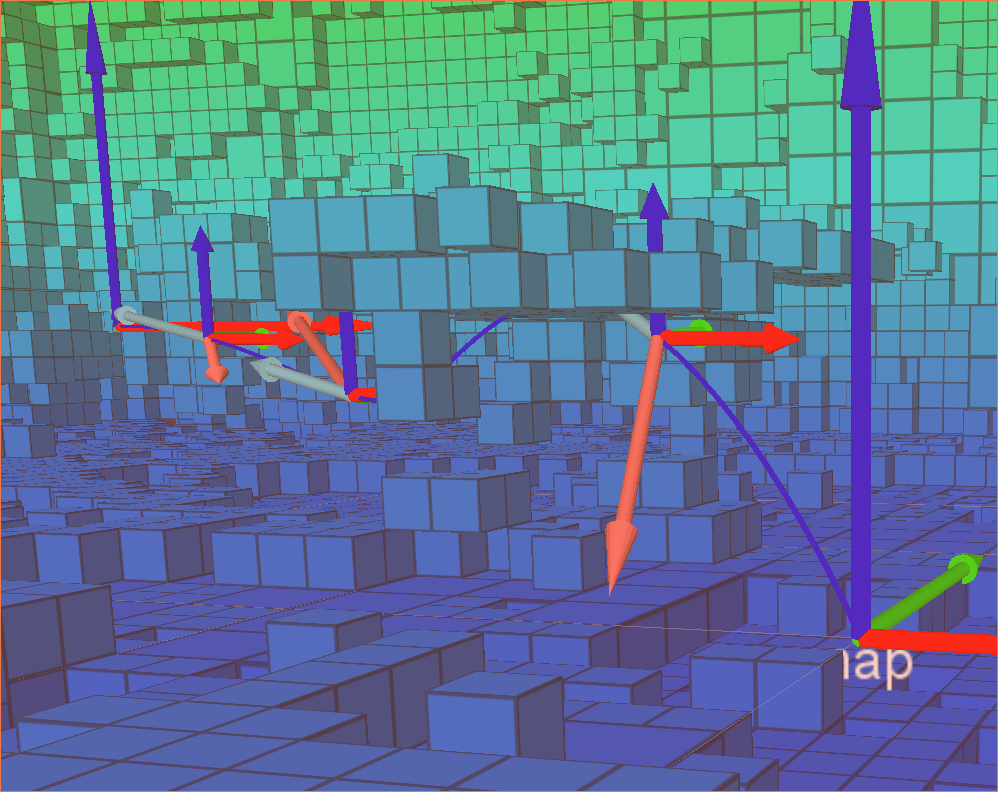
\includegraphics[width=1\textwidth]{pics/Vertex_in_middle_2.png}
   \caption{Ein Bild.}
\end{figure}

\begin{figure}[h]
   \centering
   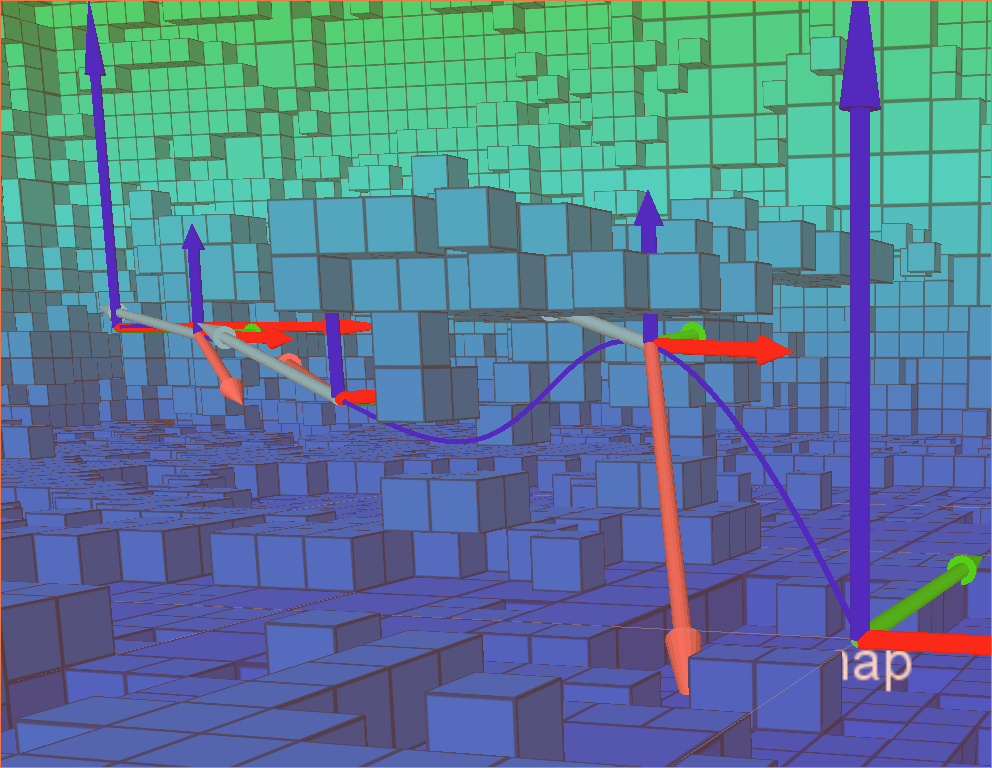
\includegraphics[width=1\textwidth]{pics/section.png}
   \caption{Ein Bild.}
\end{figure}



\begin{figure}[h]
   \centering
   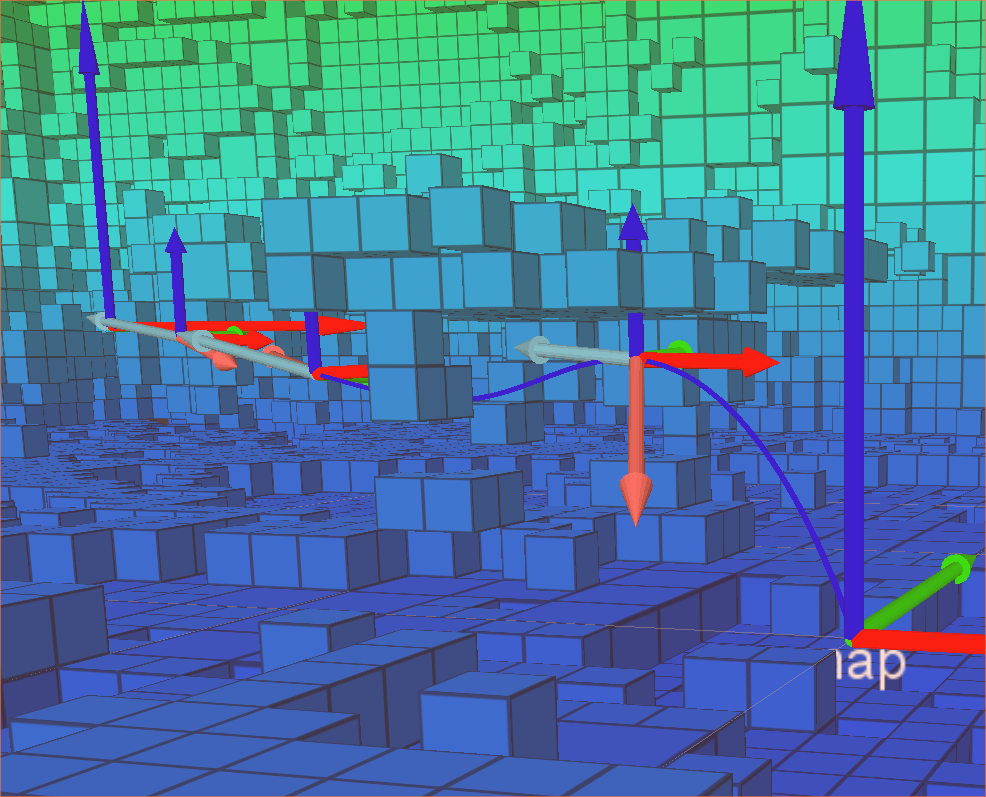
\includegraphics[width=1\textwidth]{pics/section_and_time.png}
   \caption{Ein Bild.}
\end{figure}


\begin{figure}[h]
   \centering
   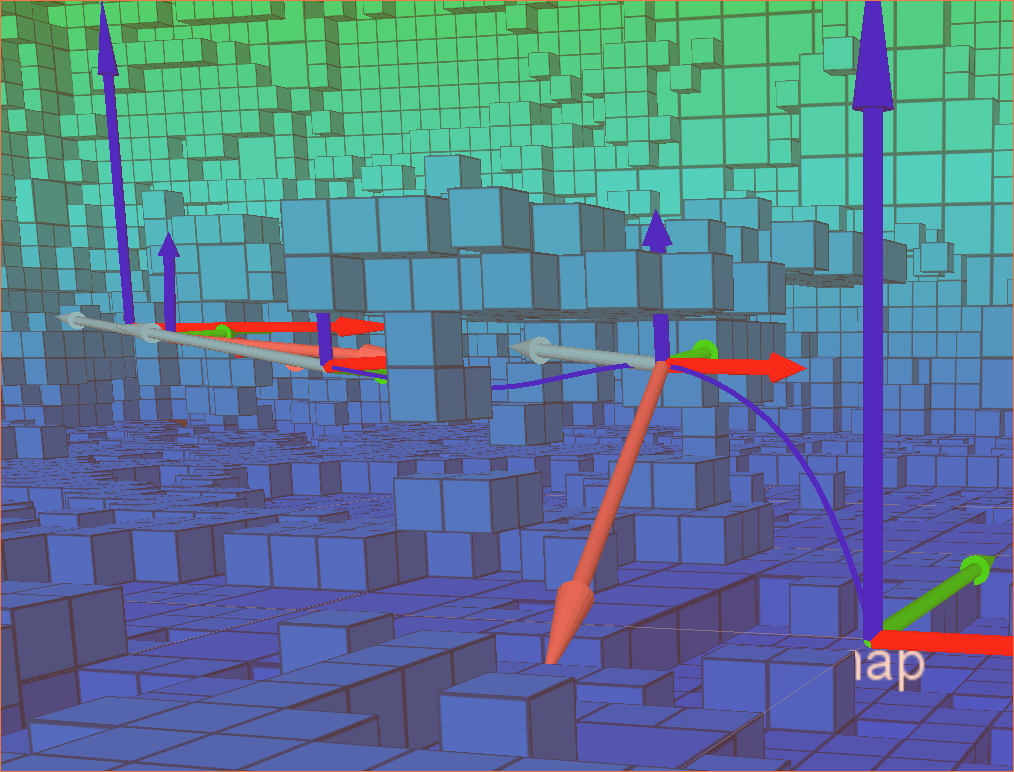
\includegraphics[width=1\textwidth]{pics/Nlopt_after_sectionAndTime.png}
   \caption{Ein Bild.}
\end{figure}